\documentclass[lang=cn,10pt,newtx]{elegantbook}
\usepackage{tikz}
\usepackage{float}
\newtheorem{Thm}{\hspace{2em}定理}[section]
\newcommand{\supp}{\text{supp}}
\newcommand{\dif}{\mathrm{d}}
\newcommand{\avg}[1]{\left\langle #1 \right\rangle}
\newcommand{\difFrac}[2]{\frac{\dif #1}{\dif #2}}
\newcommand{\pdfFrac}[2]{\frac{\partial #1}{\partial #2}}
\newcommand{\OFL}{\mathrm{OFL}}
\newcommand{\UFL}{\mathrm{UFL}}
\newcommand{\fl}{\mathrm{fl}}
\newcommand{\op}{\odot}
\newcommand{\cp}{\cdot}
\newcommand{\Eabs}{E_{\mathrm{abs}}}
\newcommand{\Erel}{E_{\mathrm{rel}}}
\newcommand{\DR}{\mathcal{D}_{\widetilde{LN}}^{n}}
\newcommand{\add}[2]{\sum_{#1=1}^{#2}}
\newcommand{\innerprod}[2]{\left<#1,#2\right>}
\newcommand\tbbint{{-\mkern -16mu\int}}
\newcommand\tbint{{\mathchar '26\mkern -14mu\int}}
\newcommand\dbbint{{-\mkern -19mu\int}}
\newcommand\dbint{{\mathchar '26\mkern -18mu\int}}
\newcommand\bint{
{\mathchoice{\dbint}{\tbint}{\tbint}{\tbint}}
}
\newcommand\bbint{
{\mathchoice{\dbbint}{\tbbint}{\tbbint}{\tbbint}}
}
\title{Note For Finite Element Methods}
\subtitle{Zhejiang University}

\author{Shuang Hu}
\institute{Zhejiang University}
\date{Sept 14, 2022}
\version{1.0}
\bioinfo{简介}{2022秋冬学季“有限元方法”课程笔记}

\setcounter{tocdepth}{3}

\logo{logo-blue.png}
\cover{cover.jpg}

% 本文档命令
\usepackage{array}
\newcommand{\ccr}[1]{\makecell{{\color{#1}\rule{1cm}{1cm}}}}

% 修改标题页的橙色带
\definecolor{customcolor}{RGB}{32,178,170}
\colorlet{coverlinecolor}{customcolor}
\usepackage{cprotect}

\addbibresource[location=local]{reference.bib} % 参考文献,不要删除

\begin{document}

\maketitle
\frontmatter

\tableofcontents

\mainmatter

\chapter{引入}
\section{为什么需要有限元方法?}
此前在《微分方程数值解》课程中,我们已经学习了有限差分法和有限体积法。这两种方法有不少优点:首先,比较直观,只要知道如何利用差分近似导数即可得到对应的差分公式;其次,在一些情形下,有限差分和有限体积方法可以实现较高的计算精度。

但是,这两种算法有一些明显的缺陷。
\begin{itemize}
  \item 算法稳定性的分析比较复杂。
  \item 处理不规则区域的问题时较为麻烦,需要多次利用插值近似。
  \item 只是求解离散格点的近似点值/离散网格的近似积分平均值,未能给出函数整体的近似。
\end{itemize}

为此,基于函数逼近论的\textbf{有限元方法}被提出。该算法能弥补有限差分法的一些明显缺陷,目前是最主流的数值算法之一。
\section{从一维边值问题说起}
考虑如下例子:
\begin{equation}
  \label{eq:ode1}
  \left\{
    \begin{aligned}
    -u''+u&=f(x),x\in(0,1)\\
    u(0)=u(1)&=0.
    \end{aligned}
  \right.
\end{equation}
类似于“偏微分方程”课程中对弱解的讨论方式,在\eqref{eq:ode1}两边同时乘某个函数$v$并在$[0,1]$上积分,得到如下形式:
\begin{equation}
  \label{eq:bianfen}
  \int_{0}^{1}(-u''+u)v\dif x=\int_{0}^{1}fv\dif x.
\end{equation}
定义函数空间$V$如下:
\begin{equation}
  \label{eq:sobolev1-1}
  V:=\left\{v\left.\right|v(0)=v(1)=0,\int_{0}^{1}((v')^{2}+v^{2})\dif x<\infty\right\}.
\end{equation}
如果函数$v\in V$, 利用分部积分法,\eqref{eq:ode1}可以转化为以下问题:
\begin{example}
  \label{ex:equiv1}
  记$a(u,v)=\int_{0}^{1}(u'v'+uv)\dif x$, $h(v)=\int_{0}^{1}fv\dif x$, $v\in V$.求$u\in V$,使得$a(u,v)=h(v)$ $\forall v\in V$.
\end{example}
下面的定理说明了该问题可以转化为一个优化问题:
\begin{theorem}{}{}
  \label{thm:bianfen}
  记泛函$J(v):=\frac{1}{2}a(v,v)-h(v)$,问题\ref{ex:equiv1}与最小化$J(v)$的优化问题等价。即:如果$a(u,v)=h(v)\forall v\in V$, 那么$J(u)\le J(v)\forall v\in V$。
\end{theorem}
\begin{proof}
  $\Rightarrow$:
  \begin{equation}
    \label{eq:dif}
    \begin{aligned}
      J(v)-J(u)&=\frac{1}{2}a(v,v)-h(v)-\frac{1}{2}a(u,u)+h(u)\\
      &=\frac{1}{2}(a(v,v)-a(u,u)-2h(v-u))\\
      &=\frac{1}{2}(a(v,v)-a(u,u)-2a(u,v-u))\\
      &=\frac{1}{2}(a(v,v)+a(u,u)-2a(v,u))\\
      &=\frac{1}{2}(a(v-u,v-u))\ge0.
    \end{aligned}
  \end{equation}
  由\eqref{eq:dif}可得,如果$a(u,v)=h(v)$,那么$J(u)\le J(v)$.

  $\Leftarrow$: $\forall v\in V$, $t\in\mathbb{R}$,有$J(u+tv)\ge J(u)$。我们定义函数$g(t):=J(u+tv)$,根据上面的讨论可知:$g'(0)=0$。另一方面,计算$g(t)$的表达式,有:
  \begin{equation}
    \begin{aligned}
      \label{eq:gt}
      g(t)&=J(u+tv)\\
      &=\frac{1}{2}\int_{0}^{1}((u'+tv'
      )^{2}+(u+tv)^{2})\dif x-\int_{0}^{1}f(u+tv)\dif x\\
    \end{aligned}
  \end{equation}
  对\eqref{eq:gt}求一阶导数,可得:
  \begin{equation}
    \label{eq:dirg0}
    g'(0)=\int_{0}^{1}(u'v'+uv)\dif x-\int_{0}^{1}fv\dif x.
  \end{equation}
  根据$g$的一阶条件,可得$a(u,v)=h(v)$。又由于$v$的任意性,结论得证。
\end{proof}

如此,我们把一个解微分方程的问题,利用\ref{ex:equiv1}和\ref{thm:bianfen}转化为了一个变分问题。由于$V$是一个无穷维空间,我们不能期望利用算法给出这个变分问题的精确解,但我们可以考虑对空间$V$进行有限维近似,并在有限维空间上近似求解这个变分问题。

\section{有限元思想的导出}
接下来,根据上一节的思路,我们继续问题\eqref{eq:ode1}的近似求解。根据上面的分析,我们的数值算法需要解决两个问题:
\begin{itemize}
  \item 如何对函数空间$V$进行有限维近似?
  \item 在进行有限维近似之后,如何在有限维空间中对变分问题进行求解?
\end{itemize}
首先,我们考虑第二个问题。根据上面的讨论,近似求解变分问题有两种不同的思路,分别对应的是\textbf{Galerkin近似方法}和\textbf{Ritz近似方法}。
\subsection{Galerkin近似}
\textbf{假设已经给出有限维子空间}$V_{N}\le V$,Galerkin近似的目的是求解$u_{N}\in V_{N}$使得
\begin{equation}
  \label{eq:Galerkin}
  a(u_{N},v_{N})=h(v_{N})
\end{equation}
对所有$v_{N}\in V_{N}$都成立。

由于$V_{N}$是有限维的空间,我们可以找到这个空间中的一组基函数$\{\phi_{1},\cdots,\phi_{N}\}$,注意到$a(u,v)$是对称双线性函数,设$u_{N}=\alpha_{1}\phi_{1}(x)+\cdots+\alpha_{N}\phi_{N}(x)$,$v_{N}(x)=\phi_{i}(x)$,代入\eqref{eq:Galerkin},可得一个线性方程组:
\begin{equation}
  \label{eq:LinearSystem}
  \begin{bmatrix}
    a(\phi_{1},\phi_{1})&a(\phi_{1},\phi_{2})&\cdots&a(\phi_{1},\phi_{N})\\
    a(\phi_{2},\phi_{1})&a(\phi_{2},\phi_{2})&\cdots&a(\phi_{2},\phi_{N})\\
    \vdots&\vdots&\ddots&\vdots\\
    a(\phi_{N},\phi_{1})&a(\phi_{N},\phi_{2})&\cdots&a(\phi_{N},\phi_{N})\\
  \end{bmatrix}
  \begin{bmatrix}
    \alpha_{1}\\
    \alpha_{2}\\
    \vdots\\
    \alpha_{N}\\
  \end{bmatrix}
  =\begin{bmatrix}
    h(\phi_{1})\\
    h(\phi_{2})\\
    \vdots\\
    h(\phi_{N})\\
  \end{bmatrix}
\end{equation}
解这个线性方程组,得到系数向量,即可给出该方程的近似解。

\subsection{Ritz方法}
同样,假设有限维子空间$V_{N}\le V$已经给出,\textbf{Ritz方法}的思路是求解有关$J(u)$的优化问题,即:求$u_{N}\in V_{N}$,使得
\begin{equation}
J(u_{N})\le J(v)\forall v\in V_{N}.
\end{equation}
这里$J(v):=\frac{1}{2}a(v,v)-h(v)$。

给出这个问题之后,我们在有限维空间中,利用最优化算法求解该问题。

这两个思路都是建立在有限维子空间$V_{N}$已经给出的前提下的。但这个有限维空间如何构造?

一个很容易想到的思路是利用$v(0)=v(1)$这一性质,构造三角函数系作为基底。这种选取思路对于问题\eqref{eq:ode1}而言当然是极好的,三角函数系的正交性也使得\eqref{eq:LinearSystem}中的系数矩阵变得相当简单易求解。但这个方案的可扩展性并不强,如果扩展到二维平面上,乃至更高维度的椭圆偏微分方程,就很难找到像这样全局定义的基函数。如果问题区域非规则或是存在不同方程的耦合,则更是如此。

\textbf{有限元方法}由此引出。
\section{有限元方法}
在上面两种思路的基础上,我们需要一个方便推广的构建有限维子空间的方法。

多项式函数空间是最容易表示的函数空间,因此这是我们的首选。但全局定义的多项式很难保证其符合边界条件。于是,借助样条插值的思想,我们转为考虑分段多项式空间。

\subsection{线性有限元空间}
我们先针对问题\eqref{eq:ode1},考虑最简单的近似形式--分段线性近似。在这种情形下,有限维子空间$V_{h}$由$(0,1)$上的分段线性函数表示。
\begin{definition}{线性有限元空间}
  \label{LinearFE}
  线性有限元空间的定义为:
  \begin{equation}
    \label{eq:linearFE}
    V_{h}:=\{v_{h}\in C(0,1):v_{h}(0)=v_{h}(1)=0,v_{h}|_{[x_{i},x_{i+1}]}\in\mathbb{P}_{1}\}.
  \end{equation}
  其中$\{x_{i}\}_{i=0}^{n}$为$[0,1]$上给定的互异节点,$x_{0}=0$,$x_{n}=1$。
\end{definition}
首先需要讨论的是,空间$V_{h}$的维数和基底。空间\eqref{eq:linearFE}的形式很容易联想到数值分析课程中学习过的\textbf{B-样条空间}。特别地,一维B-样条基函数为所谓的“hat-function”,定义如下:
\begin{equation}
  \label{eq:hatfunc}
  \phi_{i}(x)=\left\{
    \begin{aligned}
      &\frac{x-x_{i-1}}{x_{i}-x_{i-1}},x_{i-1}\le x\le x_{i}\\
      &\frac{x_{i+1}-x}{x_{i+1}-x_{i}},x_{i}\le x\le x_{i+1}\\
      & 0,otherwise\\
    \end{aligned}
  \right.
\end{equation}
\begin{figure}[H]
  \centering
  \caption{hat函数的示意图}
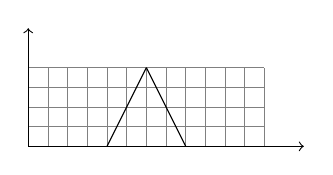
\begin{tikzpicture}
  \draw[step=.25cm,gray,very thin] (0,0) grid (3,1); 
  \draw [->](0,0) -- (3.5,0); 
  \draw [->](0,0) -- (0,1.5); 
  \draw (1,0) -- (1.5,1);
  \draw (1.5,1) -- (2,0);
\end{tikzpicture}
\end{figure}
容易验证,如此定义的$(\phi_{1},\cdots,\phi_{n-1})$构成了空间$V_{h}$的一组基。从而可得$\dim(V_{h})=n-1$。
\end{document}
